% Preamble
% ---
\documentclass{article}


% Packages
% ---
%\usepackage{amsmath} % Advanced math typesetting
\usepackage[utf8]{inputenc} % Unicode support (Umlauts etc.)
\usepackage[ngerman]{babel} % Change hyphenation rules
\usepackage{hyperref} % Add a link to your document
\usepackage{graphicx} % Add pictures to your document
\usepackage{listings} % Source code formatting and highlighting
\usepackage{caption}
\usepackage{subcaption}

\graphicspath{ {./img/} }

\begin{document}

    \author{Federico Rachelli}
    \title{\vspace{-2cm}DataVirus.it}
    \maketitle

    L'app \textbf{\href{https://datavirus.it}{DataVirus.it}} é ispirata dal sito web omonimo.
    Fornisce all'utente una visualizzazione grafica dei dati del Dipartimento di Protezione Civile sull'andamento dell'epidemia di COVID-19.
    \\
    I dati sono accedibili dal \href{https://github.com/pcm-dpc/COVID-19}{repository GitHub ufficiale} della Protezione Civile. 
    Tali dati sono aggiornati quotidianamente (a partire dalle ore 18:00) fino alla fine dello stato di emergenza dichiarato dal Consiglio dei Ministri in data 31 Gennaio 2020.
    
    \section{Funzionamento dell'applicazione}
    L'applicazione all'avvio visualizza una schermata di caricamento dei dati dal Dipartimento di Protezione Civile. 
    Tali dati, una volta ottenuti, sono elaborati e vengono mostrati all'utente gli andamenti a livello nazionale dell'epidemia.
    
    \begin{figure}[h]
        \centering
        \begin{subfigure}{.5\textwidth}
          \centering
          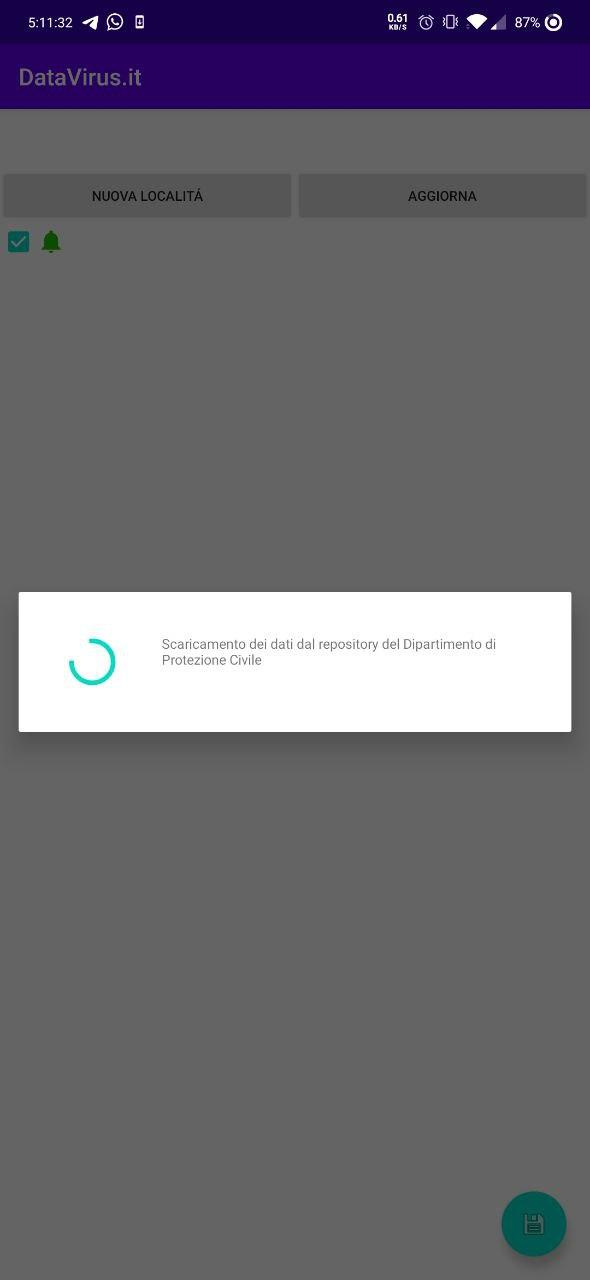
\includegraphics[width=.7\linewidth]{loading_dialog.jpg}
          \caption{Caricamento dei dati}
          \label{fig:sub1}
        \end{subfigure}%
        \begin{subfigure}{.5\textwidth}
          \centering
          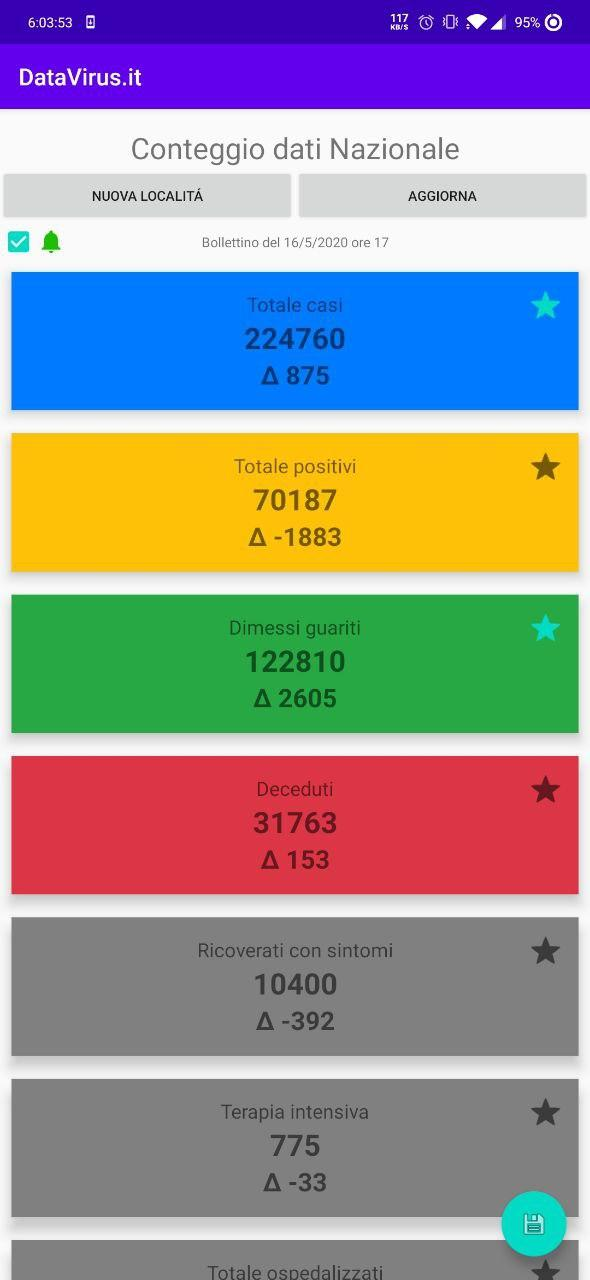
\includegraphics[width=.7\linewidth]{main_activity.jpg}
          \caption{Andamento nazionale}
          \label{fig:sub2}
        \end{subfigure}
        \label{fig:test}
    \end{figure}
        

\end{document}